\documentclass{ctexart}

\usepackage{geometry}

\geometry{a4paper, right=3cm, left=3cm, top=2cm, bottom=2cm}

\usepackage{color}
\usepackage{soul}
\usepackage{amsmath}
\usepackage[british]{babel}
\usepackage[utf8]{inputenc}
\usepackage{epstopdf}
\usepackage{csquotes}
\usepackage[hidelinks]{hyperref}
\usepackage[
    style=apa,
    backend=biber,
    sortcites=true,
    sorting=nyt,
%    isbn=false,
%    url=false,
%    doi=false,
%    eprint=false,
    hyperref=false,
    backref=false,
%    firstinits=false,
]{biblatex}

% maps apacite commands to biblatex commands
\let \citeNP \cite
\let \citeA \textcite
\let \cite \parencite

\bibliography{reference}

\usepackage[T1]{fontenc}

% Required for inserting images
\usepackage{graphicx} 

\pagestyle{plain} % 页码放下面
\title{Semantics and Syntax of Degree Construction in and Mandarin}
\date{\vspace{-10ex}}

\usepackage{enumitem}
\setlist[enumerate,1]{label=(\arabic*)}
\setlist[enumerate,2]{label=(\alph*)}

%%%%%%%%%%%%%%%%%%%%%%%%%%%%%%%%%%%%%%%%%%%%%%%%%%%

\begin{document}

\thispagestyle{empty} % 这一页清空

\begin{center}

Name: $<<$* Zhang Yi Feng *$>>$ \\
Student ID: $<<$* 1155166448 *$>>$

\end{center}

{\let\newpage\relax\maketitle}

% 简介一下比较,给出中英例子,中文比较级分类
% 主要要说明清楚,positive comparative 这几个分类

\section{Introduction}

\setcounter{page}{1}

Gradability is an essential concept in the studies of adjectives, which classifies adjectives into two major classes, non-gradable adjectives, like \textit{British}, etc. and gradable adjectives, like \textit{tall}, \textit{long}, etc. Gradable adjectives are important role to build degree comparative constructions in a language. In this section, this paper will go through a batch of examples of comparatives and categorize them by their different structures, and this classification will lead semantic and syntactic analysis in next sections. 

A simplest example in English is shown in \ref{degree_construction_example}, in this sentence, word "\textit{than}" is a comparative marker whose job is introduce strict partial relation meaning "greater than" \hl{ref here}, and suffix "-\textit{er}" is another comparative marker whose function is still controversial. Some researchers believe that "-\textit{er}" is just a word in specifier position without crucial function \cite{von1984a,heim1985,bhatt2004,rullmann1995}, another kind of view treat this word as a head of Degree Phrase(DegP) \cite{bierwisch1989,corver1990,corver1993,corver1997a,kennedy1997,grano2012}. Different form English, Mandarin is considered as a single mark language in comparative expression \cite{bobaljik2012,grano2012}. In most of cases, this mark is morpheme "\textit{bi}" such as example in \ref{degree_construction_example_Mandarin}, and there is no inflection of adjectives in Mandarin like "-\textit{er}" in English \cite{guo2012}. 

\begin{enumerate}
    \item \label{degree_construction_example}
    John is taller than Mary.
\end{enumerate}

\begin{enumerate}[resume]
    \item \label{degree_construction_example_Mandarin}
    John bi Mary gao.  \\
    \textit{John than Mary tall.} \\
    John is taller than Mary.
\end{enumerate}

Another important part of comparative structure is differential phrase(DP), whose job is giving the differential scale of context individuals. A comparative structure with differential phrase in English is shown in \ref{degree_construction_dp_example}, and Mandarin version is shown in \ref{degree_construction_dp_example_Mandarin}.

\begin{enumerate}[resume]
    \item \label{degree_construction_dp_example}
    John is 2 meters taller than Mary.
\end{enumerate}

\begin{enumerate}[resume]
    \item \label{degree_construction_dp_example_Mandarin}
    John bi Mary gao 2 mi.  \\
    \textit{John than Mary tall 2 meters.} \\
    John is 2 meters taller than Mary.
\end{enumerate}

The differential phrase in examples above are specific differential phrase, which give a accurately value of scale about gradable adjective. Another type of differential phrase gives vague value of scale. When this kind of differential phrase appears in comparative meaning, there is always a standard scale existed in context, and this vague value is either bigger than the standard value, or smaller than the standard value. Like example in \ref{dp_big_vague_example}, morpheme "\textit{hen duo}" is a big value vague differential phrase, which means, John is not only taller than Mary, but also, the difference of their height is lager than a standard value. This standard value is given in context, it is a consensus between speakers. Similarly, a small value vague differential phrase is shown in \ref{dp_small_vague_example}. In Mandarin, vague differential phrase can be complex, many researchers \cite{lin2014,li2015} do deeply investigation on it, \ref{dp_value_big_vague_example} and \ref{dp_value_small_vague_example} show such type of differential phrase which appears as "vague prefix + accurately value" or "accurately + vague suffix".

\begin{enumerate}[resume]
    \item
    \begin{enumerate}[ref=(\arabic{enumi}\alph*)]
        \item \label{dp_big_vague_example}
        John bi Mary gao hen duo.\\
        \textit{John than Mary tall much.} \\
        John is much taller than Mary.

        \item \label{dp_small_vague_example}
        John bi Mary gao yi dian.\\
        \textit{John than Mary tall a little.}\\
        John is a little taller than Mary.

    \end{enumerate}
\end{enumerate}

\begin{enumerate}[resume]
    \item
    \begin{enumerate}[ref=(\arabic{enumi}\alph*)]
        \item \label{dp_value_big_vague_example}
        John bi Mary gao liang mi duo.\\
        \textit{John than Mary tall 2 meters more.} \\
        John is more than 2 meters taller than Mary.

        \item \label{dp_value_small_vague_example}
        John bi Mary gao bu dao liang mi.\\
        \textit{John than Mary tall less 2 meters.} \\
        John is less than 2 meters taller than Mary.
    \end{enumerate}
\end{enumerate}

In comparative structure built by gradable adjectives, sometimes, the compare target is not a specific individual. This paper propose that there are three categories of compare target, which are "single individual comparison", "individual set comparison" and "specific value comparison". All examples mentioned above is single individual comparison. \ref{specific_value_comparison_example} gives a example of specific value comparison, in which compare target is not a individual. \ref{individual_set_comparison_example} shows a example of individual set comparison, and when it comes to compare with a individual set, the expression of sentence is changing from comparative meaning to superlative meaning.

\begin{enumerate}[resume]
    \item
    \begin{enumerate}[ref=(\arabic{enumi}\alph*)]
        \item \label{specific_value_comparison_example}
        John bi 2 mi gao.\\
        \textit{John than 2 meters tall.} \\
        John is taller than 2 meters.

        \item \label{individual_set_comparison_example}
        zai yi ban, John zui gao.\\
        \textit{in one class, John most tall.}\\
        John is tallest in class one.

    \end{enumerate}
\end{enumerate}

Besides comparative meaning and superlative meaning, the gradable adjectives can also build positive meaning and equative meaning. \ref{positive_meaning_example} shows a positive meaning example and \ref{equative_meaning_example} provides a equative meaning example. These two types is built by gradable adjective, but they do not have comparative meaning. In traditional research \hl{ref here}, the forms of comparative structure are usually divided into four categories, which are positive form, comparative form, equative form and superlative form. But form this paper's view, there are only tow forms, positive form and comparative form. The only condition of this kind of classification is, whether the gradable adjective in sentence provides a value comparison or a value assignment, namely:

\begin{itemize}
    \item[1.] A degree structure is comparative form if and only if this form's gradable adjective express "comparison" meaning.
    \item[2.] A degree structure is positive form if and only if this form's gradable adjective express "assignment" meaning.
\end{itemize}

Under this approach, \ref{positive_meaning_example} assigns a accurately value "\text{2 mi}" to another individual's height. When a scale-related group of words appears in positive form, this paper call it not differential phrase, but measure phrase(MP). Many researchers do not separate this two concepts very clear. Under out discussion, differential phrase appears in comparative form, measure phrase appears in positive form. 

\ref{equative_meaning_example} is a equative meaning structure, which gives a expression that the value of John's height is same with the value of Mary's height. The equative meaning is also kind of comparative form, because gradable adjective bear the comparison function. Here may have some controversies, someone may think that, \ref{equative_meaning_example} actually assigns the value of Mary's height to John's height, which will lead the function of gradable adjective turn to assignment. This paper argues that, the height is kind of inner property of an individual, so we can not assign one's height to another. On the opposite, the essence of equative meaning is to express a truth that, the difference between tow individuals height is zero, thus the function of gradable adjective in equative meaning is comparison rather than assignment.

Superlative meaning in \ref{individual_set_comparison_example} gives a comparison between the value of John's height and the values of others' height in class one. It is still a comparison, which makes superlative meaning classified into comparative form. Also, we can conclude a principal to depart the superlative meaning form comparative form, which is, a comparative form expresses a superlative meaning if and only if the compare target of this form is an individual set.

\begin{enumerate}[resume]
    \item
    \begin{enumerate}[ref=(\arabic{enumi}\alph*)]
        \item \label{positive_meaning_example}
        John gao 2 mi.\\
        \textit{John tall 2 meters.} \\
        John is 2 meters tall.

        \item \label{equative_meaning_example}
        John he Mary yi yang gao.\\
        \textit{John and Mary same tall.}\\
        John is as tall as Mary.

    \end{enumerate}
\end{enumerate}

Next phenomena should be noticed is the visibility of compare target. All examples above have explicit compare individual, but this target can be ignored when context has a default individual or a standard value. See example in \ref{diff_tradition_comparative_example}, in traditional research \hl{ref here}, this example is classified in positive form with positive meaning, but by this paper's approach, this example is comparative form because the gradable adjective bears the comparison function, rather than the assignment function. So the problem raises up which is that there is no compare target to comparison. Actually, there do exist a compare target under this context. The morpheme "\textit{very tall}", means that there is a standard height between speakers, and the value of John's height is greater than that standard. So this "specific value compare target" is actually a implicit compare target.

\begin{enumerate}[resume]
    \item \label{diff_tradition_comparative_example}
    John hen gao. \\
    \textit{John very tall.} \\
    John is very tall.
\end{enumerate}

Up to now, it is time to summarize all kinds classification mentioned above. First of all, a simple degree structure built by gradable adjectives can be classified into two categories, positive form and comparative form. If gradable adjectives bear value assignment function, sentence can be seen as positive form, and when gradable adjectives bear value comparison function, the degree structure can be seen as comparative form. In positive form, sentence can only express positive meaning; and in comparative form, sentence can express comparative meaning, superlative meaning or equative meaning.

In comparative form, there are three different angles to classified degree structure. 

\begin{itemize}
    \item[1.] The differential phrase is explicit or implicit.
    \item[2.] The compare target is specific value or single individual or individual set.
    \item[3.] The compare target is explicit or implicit.
\end{itemize}

After there classifications defined, there are serval rules we can conclude in Mandarin.

\begin{itemize}
    \item[1.] Explicit differential phrase and set individual compare target do not appear at same time. Because explicit differential phrase is generated between two values, one from subject and the other from compare target, but a set of individual provides much more than one.
    \item[2.] If a comparative form has explicit differential phrase and compare target is specific value, this compare target can not be implicit. Because implicit compare target always provides context standard value, which is conflict with explicit specific value.
\end{itemize}

\section{Semantic analysis in Mandarin}

\subsection{Former research about gradable adjectives}

First founder of analysis on gradable adjectives is Cresswell \cite{cresswell1976}, who creates a third primitive semantic type $d$ besides the two primitive semantic types $e$ and $t$ in classical semantics Degree semanticists also identify three major parts of gradable adjectives:

\begin{itemize}
    \item[1.] A measure function $G$, mapping the target $x$ onto the abstract dimension for measurement characteristic of the gradable adjective \cite{bartsch1974}.
    \item[2.] The total ordering relation $\geq$, which makes the set of scales corresponding to the abstract dimension ordered in pairs of a same direction.
    \item[3.] The degree variable, indicating the value of $G(x)$. A gradable adjective of predictive use is analysed as a two-place predicate with the individual and the degree as its arguments.
\end{itemize}

Since Cresswell, the semantic type of gradable adjectives is largely debated. Von Stechow proposes a comprehensive constructive analysis of comparisons \cite{von1984a}, which becomes the so-called standard analysis later \cite{bale2011}. From his view, the meaning of gradable adjectives are interpreted as a measure function and an ordering relation. The measure function maps the individual to the dimension denoted by gradable adjectives and the ordering relation ensures that the scale of the individual exceeds the degree to compare. In generative grammar, a gradable adjective is the head of adjective phrase. It functions as a two-place predicate, with an individual typed $e$ and a degree typed $d$ as its two arguments. What deserves a note is it is von Stechow who in first seriously regards degrees denoted by symbol $d$ as one of the primitive semantic types and it is degree $d$ that captures the difference between gradable adjectives and non-gradable adjectives. Here the semantic type of gradable adjectives is manifested as $<d,<e,t>>$. Still giving "\textit{tall}" as an instance, the lexical entry of a gradable adjective is shown in \ref{von_stechow_LE}, in which height denotes the measure function encoded by \textit{tall} and $\geq$ denotes the ordering relation between the individual and the degree:

\begin{enumerate}[resume]
    \item \label{von_stechow_LE} $[\![tall]\!] = \lambda d \lambda x. [height(x) \geq d]$
\end{enumerate}

The analysis of DegP headed by a degree morpheme is much more complicated. The semantic type of DegP is $<d,<e,t>>$. Based on the approach in generative grammar, DegP lands at an adjunct position of AP in the deep structure and then undergoes quantifier raising (QR) in the logical form (LF) to a node above the original IP inside which DegP is initially located, with the trace left denoting a $d$ type argument. The motivation for this movement is that, according to von Stechow’s analysis DegP can be regarded as isomorphic to a generalised quantifier phrase (QNP), an account under large debate afterwards.

The head of DegP, giving the comparative morpheme "-\textit{er}" as the typical one, takes a “than phrase” (thanP) as its complement and a differential phrase (DiffP) as its specifier. Depending on various categories of complement in thanP as well as the overt appearance, such as "\textit{2 meters}", or covert appearance of DiffP. "-\textit{er}" has kinds of semantic variants:

\begin{itemize}
\item[1.]
thanP can take three types of complement:

\begin{itemize}
\item[i.]
A direct degree expression, such as than "\textit{2 meters}", which denotes a degree argument typed $d$.
\item[ii.]
A comparative clause, such as "\textit{than Mary is tall}", which denotes a property of degree argument, typed $<d,t>$ because according to the view of Chomsky, the comparative clause \textit{than Mary is tall} owns a deep structure looking like "\textit{than} $how_i$ \textit{Mary is} $t_i$ \textit{tall}" which undergoes \textit{wh}-movement, leaving the trace $t_i$ denoting a degree variable bound by $\lambda$-operator \cite{chomsky1977}.
\item[iii.]
A bare NP, such as "\textit{than Mary}", regarded as a deletion from the full comparative clause "\textit{than Mary is tall}", also denotes a property of degree argument typed $<d,t>$.
\end{itemize}

\item[2.]
DiffP with overt appearance denotes a degree argument, typed $d$.

\end{itemize}

Here some examples of possible semantic variants of "\textit{er}" are illustrated:

\begin{enumerate}[resume]
    \item
    \begin{enumerate}[ref=(\arabic{enumi}\alph*)]
        \item \label{er_var_1} John is taller than 6 feet.
        \item \label{er_var_2} John is taller than Mary.
        \item \label{er_var_3} John is taller than Mary is.
        \item \label{er_var_4} John is 6 inches taller than Mary is.
    \end{enumerate}

\end{enumerate}

The thanP takes a direct degree expression as complement in \ref{er_var_1}, a bare NP in \ref{er_var_2}, a comparative clause in \ref{er_var_3} and \ref{er_var_4}. Optional DiffP only owns overt appearance in \ref{er_var_4}. Based on the analysis above, sematic type of "\textit{er}" in \ref{er_var_1} is $<d,<<d,t>,t>>$, in \ref{er_var_2} as well as \ref{er_var_3} is $<<d,t>,<<d,t>,t>>$, in \ref{er_var_4} is $<<d,t>,<d,<<d,t>,t>>>$.

According to type-driven computation in formal semantics, the gradable adjective typed $<d,<e,t>>$ first combines the trace of the semantic type $d$ which is left by DegP in the process of QR, then combines the subject in the matrix clause of the semantic type $e$, outputting a $t$ type proposition with a free degree variable. $\lambda$-abstraction turns this $t$ type open proposition into a property of degree typed $<d,t>$ which saturates DegP typed $<<d,t>,t>$. Finally, a $t$ type proposition is made out. Here we have successfully recapitulated the procedure in von Stechow’s analysis of how to derive a comparative construction.

The research of Kennedy investigates what the so-called gradable adjectives refer to as well as in what kind of constructions they appear, which is referred to as degree constructions in his paper\cite{kennedy1997}. In this research, Kennedy combines semantics and syntax to reveal the essence of this largely discussed topic.

As to the semantic interpretation of gradable adjectives, there are two major schools:

\begin{itemize}
    \item[1.] Scalar analyses, in which the set of scales corresponding to a gradable adjective is compatible with the partial ordering relation\cite{cresswell1976,bierwisch1989}.
    \item[2.] Vague predicate analyses, in which the extensions of gradable adjectives need to be determined according to the context\cite{ginet1973,kamp2013,klein1980}. 
\end{itemize}

Kennedy’s analysis falls into the general family of scalar analyses. However, Kennedy also makes some revolution to the classical scalar analysis, particularly as to the semantic type of gradable adjectives, as well as the interpretation of degrees.

Firstly, classical scalar analyses characterize the core meaning of gradable adjectives as an ordering relation between the target and the degree. Most scholars employing scalar approaches also believes the free variable degree to be bound by a quantificational expression\cite{hellan1981,hoeksema1983,von1984a}. In contrast, Kennedy assumes that gradable adjectives denote measure function, giving rise to his non-quantificational analysis of degree constructions.

Kennedy identifies three semantic constituents in degree constructions \cite{russell1905}: 

\begin{itemize}
    \item[1.] A reference value $G(x)$, expressing the projection from the target $x$ to the scale associated with the gradable adjective $G$.
    \item[2.] A standard value $s$, which is indicated via measure phrase or the comparative clause landing at the complement position of the preposition "\textit{than}". 
    \item[3.] Degree relation $R$, a partial ordering relation encoded by degree morphemes, elements of \{\textit{er/more, less, as, too, enough, so, how, ...}\}, which compares the reference value and the standard value. 
\end{itemize}

The formalization of degree constructions is shown in \ref{ref3}.

\begin{enumerate}[resume]
\item \label{ref3} $\lambda x.[R(G(x))(s)]$
\end{enumerate}

In terms of the syntactic structure of degree constructions, Kennedy projects the degree phrase headed by a degree morpheme as a functional phrase above the adjective phrase headed by a gradable morpheme, an account which is developed from approaches where adjectives are projected to an extended functional structure \cite{abney1987,corver1990,corver1997b,grimshaw1991}. The syntactic tree structure of degree constructions is shown in \ref{ref4}:

\begin{enumerate}[resume]
\item \label{ref4}
\end{enumerate}

\begin{figure}[h]
\centering
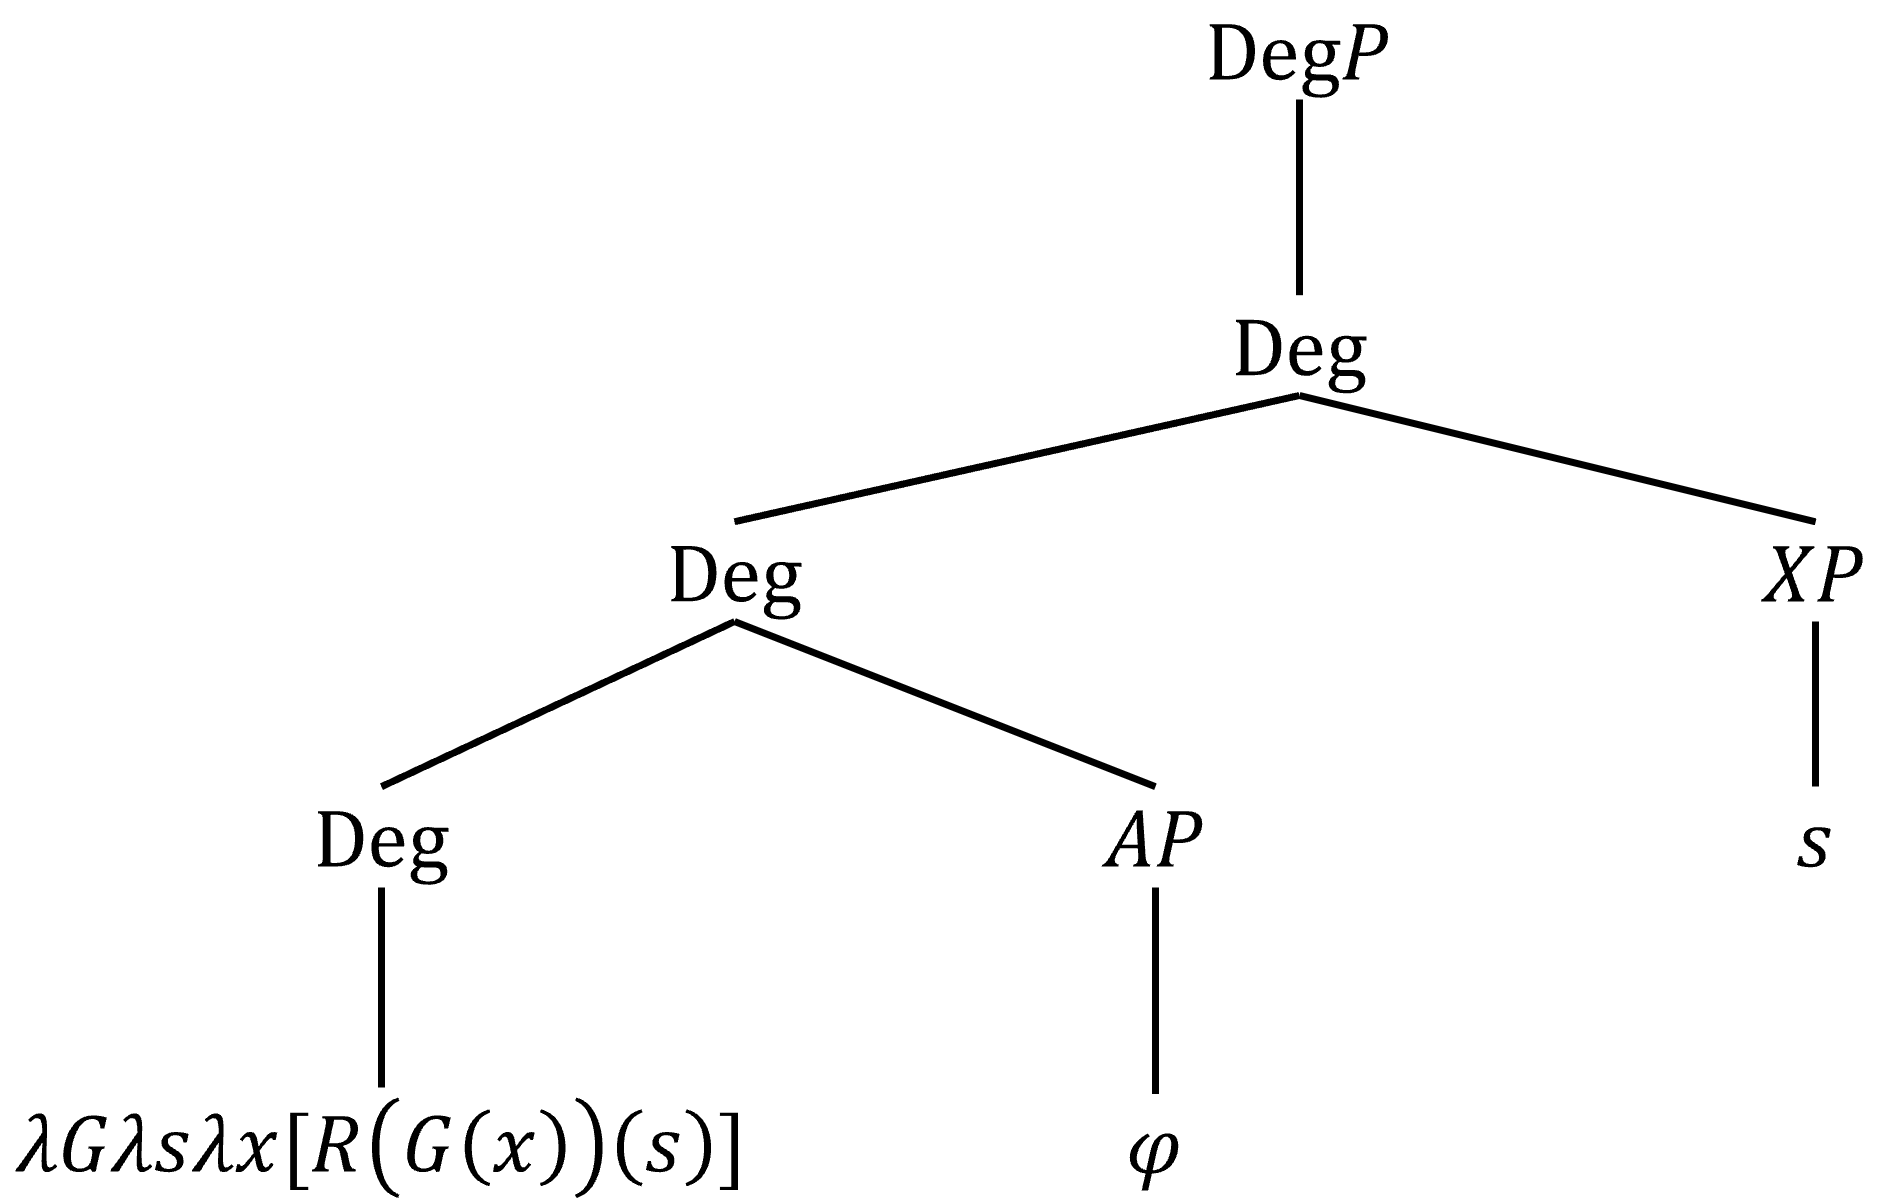
\includegraphics[width=0.5\textwidth]{pic/pic1.png}
\end{figure}

Typically, scholars think that the meaning of gradable adjectives is composed of two major parts: a measure function and an ordering relation \cite{carston2013,horn1992}.

In contrast, Kennedy’s analysis excludes the relational component from the meaning of gradable adjectives, rather assigning this semantic part to the degree morphology. This division of labour between the gradable adjective and the degree morphology is also reflected by the AP/DegP extended projection. Therefore, Kennedy’s analysis revises the semantic type of gradable adjectives from the traditional version $<d,<e,t>>$ to the simplified version $<e,t>$, making the complexity transmitted to the degree morphology.

Secondly, Kennedy makes refinement to the interpretation of degrees. He argues that degrees should be formalized as extents\cite{seuren1978,von1984b,bierwisch1989,lobner2010} rather than as points on a scale, which is different from classical scalar analyses. Based on this extent-scalar view, Kennedy assumes that gradable adjectives characteristic of adjectival polarity can be divided into positive adjectives, such as "\textit{tall}", and negative ones, such as "\textit{short}". According to this distinction, the anomaly of comparisons made between antonymous adjectives as shown in \ref{ref5} can be explained by the undefined ordering relation for extents of opposite polarity:

\begin{enumerate}[resume]
\item \label{ref5}
*Carmen is taller than Mike is short.
\end{enumerate}

\subsection{Lexical entry of gradable adjective}

In order to take a deep investigation about phenomena mentioned in last section, we shall go back to the really beginning: the lexical entry of gradable adjectives. 

There are two typical hypotheses of what this lexical entry should look like, which are shown in \ref{tallLE}. The definition of lexical entry of gradable adjectives is literally important, because different definitions of adjectives' lexical entry always lead totally different results in semantics and syntax just like Butterfly Effect.

\begin{enumerate}[resume]
    \item \label{tallLE}
    
    \begin{enumerate}[ref=(\arabic{enumi}\alph*)]
        \item \label{tallLE_a} 
        $[\![tall]\!]=\lambda d \lambda x.[Height(x) \geq d]$
    
        \item \label{tallLE_b} 
        $[\![tall]\!]=Height(x)=d$
    
    \end{enumerate}
\end{enumerate}

\ref{tallLE_a} is a traditional lexical entry of gradable adjectives, and many researchers believe in it (\colorbox{yellow}{refhere}). Under this definition, gradable adjective "\textit{tall}" is considered as a relation of "greater equal", which is true when an individual $x$ as input and $x$'s height is at least as great as $d$. A simple application of this kind of lexical entry definition to \ref{old_school_def_example} is shown in \ref{old_school_def_example_LE}.

\begin{enumerate}[resume]

    \item \label{old_school_def_example} 2 meters tall.

\end{enumerate}

\begin{enumerate}[resume]

    \item \label{old_school_def_example_LE}
    
    \begin{enumerate}[ref=(\arabic{enumi}\alph*)]
        
        \item $[\![tall]\!]=\lambda d \lambda x.[Height(x) \geq d]$
        \item $[\![2 \enspace meters \enspace tall]\!]=\lambda x.[Height(x) \geq 2 \enspace meters]$

    \end{enumerate}

\end{enumerate}

Actually, lexical entry definition like \ref{tallLE_a} remains a problem with corresponding examples shown in \ref{old_school_def_problem}. In English, sometimes measure phrase can not directly combine with negative-pole adjectives. We can say someone is "\textit{2 meters tall}", but can not say someone is "\textit{2 meters short}". But situation changes when suffix "\textit{er}" shows up in \ref{old_school_def_problem_correct}, "\textit{2 meters shorter}" is a correct usage in English. Besides, this phenomenon is also a language-specific problem, in Japanese, we can not combine measure phrase even with "\textit{segatakai}(\textit{tall})". Traditional lexical entry of gradable adjectives has no ability to explain this phenomenon.

\begin{enumerate}[resume]

    \item \label{old_school_def_problem}
    
    \begin{enumerate}[ref=(\arabic{enumi}\alph*)]
        
        \item 2 meters tall. 10 years old.
        \item *2 meters short. *10 years young.
        \item \label{old_school_def_problem_correct} 2 meters shorter. 10 years younger.

    \end{enumerate}

\end{enumerate}

Based on the problem mentioned above, there is another group of researchers propose that the gradable adjectives' lexical entry should not encode the partial ordering relation, instead, the gradable adjectives should reveal the original property of an individual, which means "\textit{tall}" should simply illustrate the height of an individual. Thus the lexical entry of gradable adjectives should looks like \ref{tallLE_b}, in which there is just a measure function. 

Under this assumption, the partial ordering relation still needs a place to be introduced, if not, there will be a lexical entry type mismatch. The type of measure function "\textit{tall}" is $<e,d>$, but measure phrase is type $d$, so gradable adjectives are no way to composite with measure phrase on account of type-theoretic. To resolve this problem, Svenonius\cite{svenonius2006} claims that there is a null operator whose semantic function is linking the lexical entry of gradable adjectives and the lexical entry of measure phrase, and syntactic function is to introduce a degree argument and bear the mission of introducing the "greater equal" meaning. The denotation of this null operator is spelled out in \ref{gao_nop_LE}, and the \ref{gao_nop_LE_c} shows the composition of null operator and gradable adjective, which is same with \ref{tallLE_a}. The lexical entry of \ref{gao_nop_LE_c} is $<d,<e,t>>$, which can combine with measure phrase with out any type conflict.

\begin{enumerate}[resume]
    \item \label{gao_nop_LE}

    \begin{enumerate}[ref=(\arabic{enumi}\alph*)]
        \item \label{gao_nop_LE_a} 
        $[\![nop]\!]=\lambda G_{<e,d>}\lambda d \lambda x.[G(x) \geq d]$

        \item \label{gao_nop_LE_b} 
        $[\![tall]\!]=Height(x)$

        \item \label{gao_nop_LE_c} 
        $\begin{aligned}[t]
            [\![nop \enspace tall]\!] &= [\![nop]\!]([\![tall]\!]) \\
            &= \lambda d \lambda x.[Height(x) \geq d]
        \end{aligned}$

    \end{enumerate}
\end{enumerate}

Although the lexical result of null operator and adjectives in \ref{gao_nop_LE_c} looks exactly same with traditional lexical entry of gradable adjectives in \ref{tallLE_a}, which makes this null operator seems redundant. But this "null operator + gradable adjective" structure resolve the problem mentioned in \ref{old_school_def_problem}. Actually, this design separates the "individual property function" from "greater equal meaning", the former's owner is gradable function, and latter's owner is null operator. It is null operator who does not select for "\textit{short"} when measure phrase is "\textit{2 meters}". And, this idiosyncratic property of null operator is language-specific. The advantage of this kind of structure is leaving language-specific problem to null operator and keeping gradable adjectives away form any idiosyncratic language-specific properties.

Next questions are, whether this null operator has a specific phonetic expression in any language and where its position is in syntactic structure. 

For the first question, Svenonius does a deep investigation about Icelandic and Norwegian, which shows that a phonetic word of this null operator does not exist in Norwegian but does exist in Icelandic. In Icelandic, \ref{Icelandic_example} gives three different ways to express the same meaning. In \ref{Icelandic_example_10}, the word "\textit{Hversu}" is mapping to two English words "\textit{how.much}", but actually "\textit{Hversu}" only used as a degree operator, and it does not bear the function of manner adverbial. In \ref{Icelandic_example_a}, speaker can omit word "\textit{Hversu}" and \colorbox{yellow}{front predicate} to express the same meaning. Also, in \ref{Icelandic_example_b}, a word "\textit{Hvað}" can be placed at the beginning of the sentence, and keep all other morphemes in their original position. What should be noticed is that the Icelandic word "\textit{Hvað}" does not have real meaning, it is just a phonologically placeholder, which exactly is an evidence of the existence of null operator. For the latter question, Svenonius gives syntactic structures of \ref{Icelandic_example} respectively as shown in \ref{Icelandic_example_LE}. From Svenonius' perspective, null operator and the word "\textit{Hvað}" show the same locality conditions which is same with famous \textit{wh}-movement. 

\begin{enumerate}[resume]
    \item \label{Icelandic_example}
    
    \begin{enumerate}[ref=(\arabic{enumi}\alph*)]
        \item \label{Icelandic_example_10}
        Hversu gammall ertu? \\
        \textit{how.much old are.you} \\
        how old are you?

        \item \label{Icelandic_example_a}
        er du gammel? \\
        \textit{are you old} \\
        how old are you?

        \item \label{Icelandic_example_b}
        Hvað ertu gammall? \\
        \textit{null are you old} \\
        how old are you?

    \end{enumerate}   
    
\end{enumerate}

\begin{enumerate}[resume]
    \item \label{Icelandic_example_LE}
    
    \begin{enumerate}[ref=(\arabic{enumi}\alph*)]
        \item $[_{CP}Nop_1 \enspace er_2[_{IP}du_3 \enspace t_2[_{VP} t_2[_{AP} t_3 \enspace t_1 \enspace gammel]]]]$
        
        \item $[_{CP}Hva$ð$_1 \enspace er_2[_{IP} \enspace -tu_3 \enspace t_2 [_{VP}t_2[_{AP}t_3 \enspace t_1 \enspace gammel]]]]$
        
    \end{enumerate}   
    
\end{enumerate}

The $<e,d>$ type gradable adjectives seems a perfect definition. But I have to point out that, both lexical entries in \ref{tallLE} may cause a mismatch between the meaning given by lexical calculation and meaning given by language common sense. 

Since there are serval kinds of ways to build a degree construction, such as positive form, comparative form and superlative form, a lexical meaning should have ability to give a interpretation of all these constructions. \ref{tallLE_a} gives a positive form example, and it's lexical entry calculation is shown in \ref{john_gao_2_mi_LE}, who uses traditional gradable adjectives lexical type in \ref{tallLE_a}. To resolve $\lambda$ reduction, the lexical entry of "\textit{tall}" needs a measure phrase with lexical entry $d$ and an individual $x$ , which are respectively "\textit{2 meters}" and "\textit{John}". "\textit{2 meters}" changes the semantic type of "\textit{tall}" from $<d,<e,t>>$ to $<e,t>$, and "\textit{John}" is input as type $e$ which makes final result to type $t$. The result of lexical entry calculation tells a truth that John's height is not only equal to 2 meters precisely, but also has a possibility to greater than 2 meters. But actually we do know that sentence in \ref{john_gao_2_mi} means John's height is 2 meters accurately, which is mismatch with the result of semantic calculation. The reason why this mistake is made is that the partial ordering relation of degree is encoded in gradable adjectives, \colorbox{yellow}{and there is no way to resolve this "greater equal"}. \ref{tallLE_b} will also lead this problem, since the lexical entry of the combination of null operator and gradable adjective is same with the lexical entry shown in \ref{tallLE_a}.

\begin{enumerate}[resume]
    \item \label{john_gao_2_mi} Jhon is 2 meters tall.
\end{enumerate}

\begin{enumerate}[resume]
    \item \label{john_gao_2_mi_LE}
    
    \begin{enumerate}[ref=(\arabic{enumi}\alph*)]
    \item \label{john_gao_2_mi_LE_a} 
    $[\![tall]\!] = \lambda d \lambda x.[Height(x) \geq d]$
    
    \item \label{john_gao_2_mi_LE_b} 
    $\begin{aligned}[t]
        [\![2 \enspace meters \enspace tall]\!] &= [\![tall]\!](2m) \\
        &= \lambda x.[Height(x) \geq 2m]
    \end{aligned}$
    
    \item \label{john_gao_2_mi_LE_c} 
    $\begin{aligned}[t]
        [\![John \enspace is \enspace 2 \enspace meters \enspace tall]\!] &= [\![tall \enspace 2m]\!](John) \\
        &= Height(John) \geq 2m
    \end{aligned}$
    
    \end{enumerate}
\end{enumerate}

To fix the problem mentioned above, I am going to modify the lexical entry of null operator, and for convenience, I will give null operator a simple name $\mu$. New lexical entry of $\mu$ is shown in \ref{mu_LE_1}, and the result lexical entry after the combination with gradable adjective "\textit{tall}" is shown in \ref{mu_LE_2}.

\begin{enumerate}[resume]
    \item \label{mu_LE}
    
    \begin{enumerate}[ref=(\arabic{enumi}\alph*)]
        \item \label{mu_LE_1}
        $[\![\mu]\!] =  \lambda G_{<e,d>}\lambda d \lambda x.[G(x) = d]$
        \item \label{mu_LE_2}
        $[\![\mu \enspace tall]\!] = \lambda d \lambda x.[Height(x) = d]$
    \end{enumerate}
\end{enumerate}

Based on this "equal meaning" lexical entry of gradable adjectives, we can solve the problem which "greater equal" meaning lexical entry can not. Applying this $\mu$'s lexical entry to Mandarin, I give a example in \ref{john_gao_2_mi_mu}, which is a positive form degree construction. The lexical calculation is shown in \ref{john_gao_2_mi_mu_LE}. The procedure of calculation is generally same with \ref{john_gao_2_mi_LE}, but because the $\mu$ has "equal meaning", the result was lead to a correct way which gives a truth that John's height is exactly 2 meters, and that is exactly what we expect to get.

\begin{enumerate}[resume]
    \item \label{john_gao_2_mi_mu} 
    Jhon gao 2 mi. \\
    \textit{Jhon tall 2 meters.} \\
    Jhon is 2 meters tall.
\end{enumerate}

\begin{enumerate}[resume]
    \item \label{john_gao_2_mi_mu_LE}
    
    \begin{enumerate}[ref=(\arabic{enumi}\alph*)]
    \item
    $[\![\mu \enspace gao]\!] = \lambda d \lambda x.[Height(x) = d]$
    
    \item
    $\begin{aligned}[t]
        [\![\mu \enspace gao \enspace 2 \enspace mi]\!] &= [\![\mu \enspace gao]\!](2m) \\
        &= \lambda x.[Height(x) = 2m]
    \end{aligned}$
    
    \item
    $\begin{aligned}[t]
        [\![John \enspace \mu \enspace gao \enspace 2 \enspace mi]\!] &= [\![\mu \enspace gao \enspace 2 \enspace mi]\!](John) \\
        &= Height(John) = 2m
    \end{aligned}$
    
    \end{enumerate}
\end{enumerate}


\subsection{Application in Mandarin}

In last section, I introduce two traditional lexical entries of gradable adjectives, and illustrate their flaws. At the end of last section, I propose my improvement of the lexical entry of gradable adjectives. In this section, I will show how this new definition work in Mandarin degree construction.

\subsubsection{Positive form}

A simple example of positive form was shown in last section in \ref{john_gao_2_mi_mu}. In Mandarin, some decorations can be added in positive form like "\textit{hen}(very)", "\textit{youdian}(a little)", 


\subsubsection{Comparative form}


Applying this $\mu$'s lexical entry to Mandarin, I give two examples in \ref{john_gao_2_mi_nop}. In \ref{john_gao_2_mi_nop_positive}, the degree construction is positive form, so the null operator does not exist, gradable adjective "\textit{gao}" composite with measure phrase "\textit{2mi}" directly, which makes final lexical entry calculation result is $Height(John)=2mi$. That gives a truth that John's height is exactly 2 meters, which is match with what we expect. When construction comes to comparative form like \ref{john_gao_2_mi_nop_comparative} with lexical entry calculation in \ref{john_gao_2_mi_nop_comparative_LE}. There will be a null operator who should combine with "\textit{gao}" first, and changes the meaning of "\textit{gao}" from "equal meaning" to "greater equal meaning". Then, the lexical entry of important comparative morpheme "\textit{bi}" is shown in \ref{john_gao_2_mi_nop_comparative_LE_bi}.

\begin{enumerate}[resume]
    \item \label{john_gao_2_mi_nop}
    
    \begin{enumerate}[ref=(\arabic{enumi}\alph*)]
        \item \label{john_gao_2_mi_nop_positive}
        Jhon ($\mu$) gao 2 mi.  \\
        \textit{Jhon ($\mu$) tall 2 meters.}    \\
        Jhon is 2 meters ($\mu$) tall.

        \item \label{john_gao_2_mi_nop_comparative}
        Jhon bi Mary (nop) gao. \\  
        \textit{Job er Mary (nop) tall.}    \\
        Jhon is taller than Mary.

    \end{enumerate}
    
\end{enumerate}

\begin{enumerate}[resume]
    \item \label{john_gao_2_mi_nop_comparative_LE}
    \begin{enumerate}[ref=(\arabic{enumi}\alph*)]
        \item $[\![tall]\!]=Height(x)=d$
        \item $[\![nop]\!]=\lambda G\lambda d \lambda x.G(x) \geq d$
        \item 
        $\begin{aligned}[t]
            [\![nop \enspace tall]\!] &= [\![nop]\!]([\![tall]\!]) \\
            &= \lambda d \lambda x.Height(x) \geq d
        \end{aligned}$ \label{john_gao_2_mi_nop_comparative_LE_bi}
        \item $[\![bi]\!]= \lambda G_{<d,<e,t>>} \lambda y \lambda x . \exists \delta > 0 \enspace s.t.[G(x,d_x^{\prime}) - G(y,d_y^{\prime})>\delta]$
        \item
        $\begin{aligned}[t]
            [\![bi \enspace nop \enspace gao]\!] &= [\![bi]\!]([\![nop \enspace tall]\!]) \\
            &= \lambda y \lambda x . \exists \delta > 0 \enspace s.t.[Height(x,d_x^{\prime}) - Height(y,d_y^{\prime})>\delta]
        \end{aligned}$
        \item
        $\begin{aligned}[t]
            [\![John \enspace bi \enspace Mary \enspace nop \enspace gao]\!] 
            &= [\![bi \enspace nop \enspace gao]\!]([\![John]\!])([\![Mary]\!]) \\
            &= \exists \delta > 0 \enspace s.t.[Height(John,d_{John}^{\prime}) \\ 
            & \qquad - Height(Mary,d_{Mary}^{\prime})>\delta]
        \end{aligned}$
    \end{enumerate}
\end{enumerate}

The second "equal meaning" lexical entry in \ref{tallLE_b} looks like a perfect solution who resolve the meaning-mismatch problem via null operator. But, I have to point out that, this "equal meaning" solution still causes some mismatch mistakes. To illustrate this conclusion more clear, we have to find out the lexical entry of comparative morpheme first. Back to example \ref{john_gao_2_mi_nop_comparative}









such as following example in \ref{equal_mistake_example}, with lexical entry calculation shown in \ref{equal_mistake_example_LE}.

\begin{enumerate}[resume]
    \item \label{equal_mistake_example}
    Jhon bi Mary (nop) gao 2 mi. \\
    \textit{Job er Mary (nop) tall 2 meters.}    \\
    Jhon is 2 meters taller than Mary.
\end{enumerate}

\begin{enumerate}[resume]
    \item \label{equal_mistake_example_LE}
    \begin{enumerate}[ref=(\arabic{enumi}\alph*)]
        \item $[\![gao]\!]=Height(x)=d$
        \item $[\![nop \enspace tall]\!] = \lambda d \lambda x.Height(x) \geq d$
        \item $[\![nop \enspace tall \enspace 2mi]\!] \lambda x.Height(x) \geq 2mi$ 
        \item $[\![biP]\!]=\lambda G \lambda x \lambda y \lambda d. \exists d_1 \exists d_2 [(G(x) \geq d_1) \land (G(y) \geq d_2) \land (d_1-d_2 \geq 2m) ]$
    \end{enumerate}
\end{enumerate} 

\section{Complex problem in Mandarin}

In last part of this paper, I give a fundamental view about simple gradable adjectives degree structures. But in Mandarin, a degree expression can be much complex. And this part, first, a important strategy to forming comparatives in Mandarin will be introduced which is called transitive comparative, and then, some of Mandarin crucial comparative morphemes and their properties will be discussed.

\subsection{Transitive degree structure}

The transitive comparative structure is a kind of special usage of gradable adjectives in Mandarin, which dost not exist in English. In transitive comparative structure, gradable adjective as predicate should accept a measure phrase, and this measure phrase must be explicit \cite{grano2012}. \ref{transitive_example} is a basic example of transitive comparatives, in this case, gradable adjective "\textit{tall}" bears same function with transitive verb and general comparative morpheme "\textit{bi}" will not appear. 

\begin{enumerate}[resume]
    \item \label{transitive_example}
    John gao 2 mi. \\
    \textit{John tall 2 meters.} \\
    John is 2 meters tall.
\end{enumerate}


\section{Conclusion}

\newpage

\printbibliography

\end{document}
